\chapter{Descripción del proyecto}

\section{MoonPhases: Diario de Observación Lunar}

Repositorio: \href{https://github.com/Angello599/MoonPhases-DevOps}{MoonPhases}.

\url{https://github.com/Angello599/MoonPhases-DevOps}

Aplicación web que combina una simulación 3D interactiva del ciclo lunar con un panel de notas donde la persona usuaria registra sus observaciones astronómicas asociadas a una fecha concreta.

\begin{figure}[H]
    \centering
    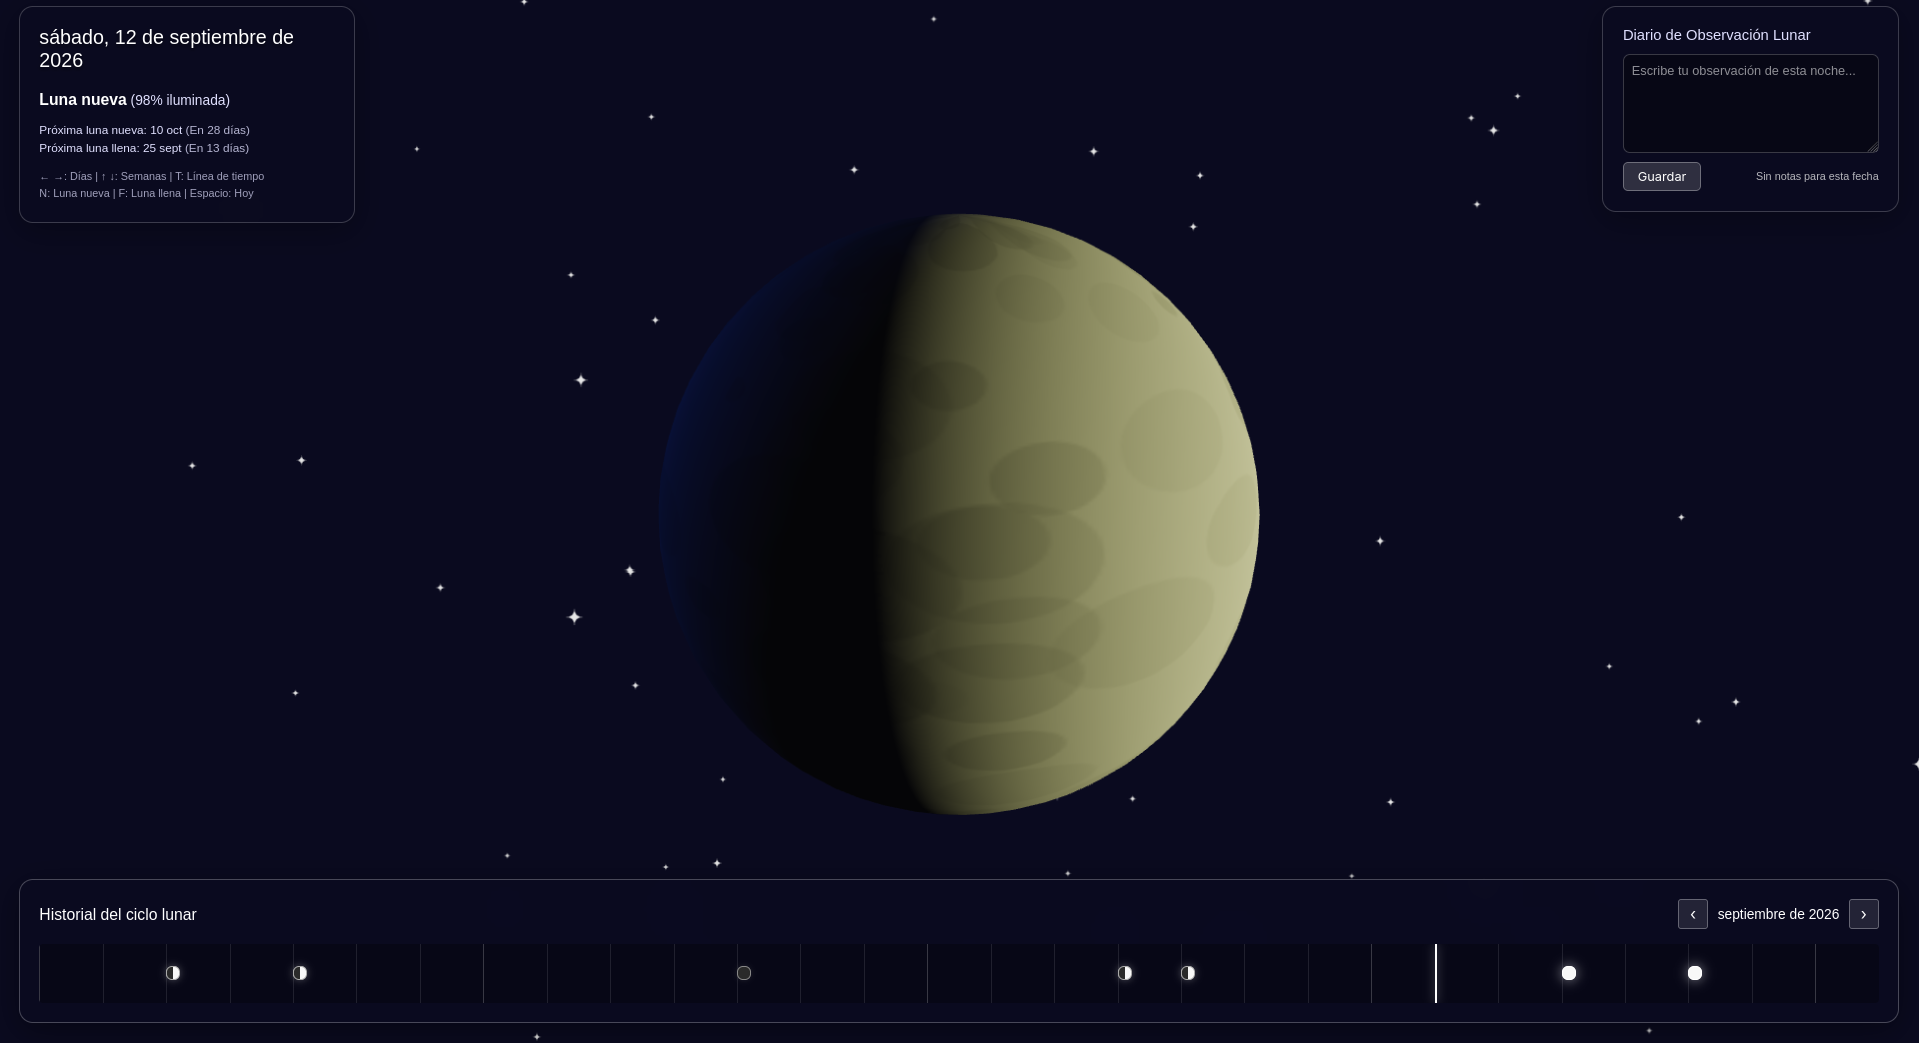
\includegraphics[width=0.92\textwidth]{content/imgs/pagina.png}
    \caption{Vista principal de la aplicación MoonPhases, con la simulación 3D del ciclo lunar y el panel de \emph{Diario de Observación Lunar}.}
\end{figure}

\subsection{Breve explicación del problema y la solución propuesta}
\emph{MoonPhases}, el proyecto original de NeaByteLab, es un simulador 3D de las fases lunares que permite recorrer el calendario y observar cómo cambia la iluminación de la luna. Sin embargo, la aplicación no permite almacenar información: el usuario no puede registrar sus observaciones ni consultarlas posteriormente.

Para resolver esta limitación, incorporamos un panel denominado \emph{Diario de Observación Lunar}, en el que el usuario puede registrar una nota asociada a una fecha y recuperarla más adelante. Para almacenar estas notas de forma persistente, reorganizamos el proyecto en tres capas:

\begin{itemize}
    \item \textbf{Frontend}: aplicación Vite + TypeScript + Three.js, servida mediante Nginx.
    \item \textbf{Backend}: API REST construida con Node.js y Express, expuesta en el puerto \texttt{3001}.
    \item \textbf{Base de datos}: PostgreSQL, con el esquema \texttt{moon\_notes} para persistir las notas.
\end{itemize}

Sobre esta base funcional, el curso de DevOps exige aplicar prácticas de control de versiones con \emph{Conventional Commits}, una metodología de \emph{branching} basada en Gitflow, y la contenerización completa de los tres servicios mediante Docker y Docker Compose, de modo que el sistema completo pueda levantarse de forma reproducible con un único comando.

\subsection{Integrantes y roles}

\begin{center}
\begin{tabularx}{\textwidth}{@{}l>{\raggedright\arraybackslash}X@{}}
\toprule
\textbf{Integrante} & \textbf{Rol dentro del proyecto} \\
\midrule
Angello Zuloaga & Adaptación del proyecto base a la arquitectura de tres capas: frontend, backend (API REST) y base de datos (esquema y conexión a PostgreSQL). \\
Eddison Pinedo & Dockerización de cada servicio (Dockerfiles, \texttt{docker-compose}), configuración de redes, volúmenes y \emph{secrets}, y documentación técnica del despliegue. \\
Nicol Campoverde & Automatización de pruebas: definición de la estrategia de pruebas unitarias y de los scripts de ejecución del proyecto. \\
\bottomrule
\end{tabularx}
\end{center}
